%------------------------------------------------
\subsection{Conclusion and future directions}
%------------------------------------------------
\begin{frame}[t]
	\frametitle{Conclusion and future directions}
	\tikzstyle{background grid}=[draw, black!50,step=.5cm]
	%
	\only<1-5>{Model discovery and development facilitated by hyperparameter optimization}%
	\only<6->{StoMADS can be improved to solve a wide variety of HPO problems}%
	\only<5>{{\color{white}\ifshowcitations\footpartcite{Hay2021}\fi}}%
	\only<7->{{\color{white}\ifshowcitations\footpartcite{Lakhmiri2019}\textsuperscript{,}\footpartcite{Bergstra2011}\fi}}\\
	%
	\tikzstyle{background grid}=[draw, black!50,step=.5cm]
	\begin{tikzpicture}[remember picture, overlay] %show background grid, 
		% Put the graphic  inside a node. This makes it easy to place the
		% graphic and to draw on top of it. 
		% The above right option is used to place the lower left corner
		% of the image at the (0,0) coordinate. 
		\node [inner sep=0pt,above left, opacity=1.0]  at (1.01\textwidth,-0.73\textheight) (prediction) 
			{
				\only<3->{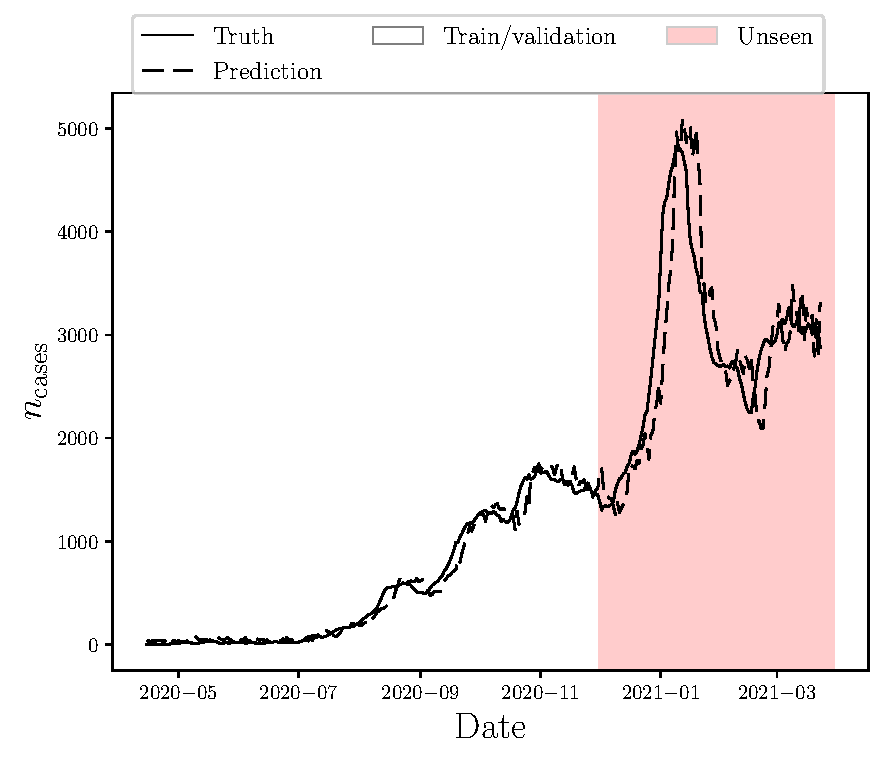
\includegraphics[width=0.5\textwidth]{predictions/model_predictions_unseen_SVR_mean_Ct_daily_cases_G12.pdf}}%
			};
		% show origin
		% \fill (0,0) circle (2pt);
	\end{tikzpicture}%
	
	\begin{columns}[c] % The "c" option specifies centered vertical alignment while the "t" option is used for top vertical alignment
		\begin{column}{.5\textwidth} % Left column and width
			\vspace{-0.0em}
			% Optimization problem
			\begin{itemize}\itemsep0em
			\only<-5>{
				\item<2-5> Cycle Threshold (Ct) is a useful feature for incidence projection
				\item<3-5> Model that generalizes well on unseen data
    			\item<4-5> Simpler models perform well when historical data is limited
				\item<5> Works well on other datasets\footnotemark[1]
			}
			\item<6-> Can be used to meet deployment targets
				\begin{exampleblock}{Objective and constraints}
					\vspace{-1.0em}%
					\begin{equation*}
						\begin{aligned}
							& \underset{\mathbf{x}}{\text{min}}
							& & f(\mathbf{x}) = \mathbb{E}_{\Theta}\left[{f}_{\Theta}(\mathbf{x}) = \mathrm{error}_\mathrm{CV}\right]\\
							& \text{subject to}
							& & {c}(\mathbf{x}) = \mathrm{\small inference~time} - \mathrm{\small threshold} \le 0\\
							& \text{where}
							& & \Theta\mathrm{:realizations}
						\end{aligned}
					\end{equation*}
				\end{exampleblock}
				\item<7-> Should be benchmarked against HyperNOMAD\footnotemark[1], Bayesian optimization\footnotemark[2]
				\item<8-> Mixed variable version is needed
			\end{itemize}
			\only<-5>{\vspace{-10em}}
		\end{column}
		%
		\begin{column}{.5\textwidth} % Left column and width
		\end{column}
	
	\end{columns}
	%
	\vspace{-3em}
\end{frame}
\addtocounter{footnote}{-2}
